\chapter{45GS02 Microprocessor}
\label{cha:cpu}
\label{cha:45gs02}
\section{Introduction}

The 45GS02 is an enhanced version of the processor portion of the CSG4510
and of the F018 "DMAgic" DMA controller used in the Commodore 65
computer prototypes.  The 4510 is, in turn,
an enhanced version of the 65CE02.
The reader is referred to
the considerable documentation available for the 6502 and 65CE02 processors
for the backwards-compatible operation of the 45GS02.

This chapter will
focus on the differences between the 45GS02 and the earlier 6502-class
processors, and the documentation of the many built-in memory-mapped I/O
registers of the 45GS02.

\section{Differences to the 6502}

The 45GS02 has a number of key differences to earlier 6502-class processors:

\subsection{Supervisor/Hypervisor Privileged Mode}

Unlike the earlier 6502 variants, the 45GS02 has a privileged mode of operation.
This mode is intended for use by an operating system or type-1
hypervisor.  The ambiguity between
operating system and Hypervisor on the MEGA65 stems from the fact that the operating
system of the MEGA65 is effectively little more than a loader and
task-switcher for C64 and C65
environments, i.e., effectively operating as a hypervisor, but provides
only limited virtualisation
of the hardware.

The key differences between normal and supervisor mode on the MEGA65, are that in
supervisor mode:

\begin{itemize}
\item A special 16KB memory area is mapped to \$8000 - \$BFFF, which is
 used to contain both
 the program and data of the Hypervisor / supervisor program.
 This is normally the Hyppo program.
  This memory is not mappable by any means when the processor is in the
 normal mode (the chip-select
  line to it is inhibited), protecting it from accidental or malicious access.
\item The 64 SYSCALL trap registers in the MEGA65 I/O-mode at
\$D640 - \$D67F are replaced by the
  virtualisation control registers.  These registers allow complete
control over the system, and
  it is their access that truly defines the privilege of the supervisor mode.
  \item The processor always operates at full speed (40MHz) and in the
 4510 processor personality.
\end{itemize}

The Hypervisor Mode is described in more detail later in this appendix.

\subsection{6502 Illegal Opcodes}

The 65C02, 65CE02 and CSG4510 processors extended the original 6502 processor
by using previously unallocated opcodes of the 6502 to provide additional
instructions.  All software that followed the official documentation of the 6502
processor will therefore work on these newer processors, possibly with different
instruction timing.  However, the common practice on the C64 and other home computers
of using undefined opcodes (often called ``illegal opcodes'', although there is no
law against using them), means that many existing programs will not work on these
newer processors.

To alleviate this problem the 45GS02 has the ability to switch processor personalities
between the 4510 and 6502.  The effect is that in 6502 mode, none of the new opcodes of
the 65C02, 65CE02, 4510 or 45GS02 are available, and are replaced with the original,
often strange, behaviour of the undefined opcodes of the 6502.

WARNING: This feature is incomplete and untested.  Most undocumented
6502 opcodes do not operate correctly when the 6502
personality is enabled.

\subsection{Read-Modify-Write Instruction Bug Compatibility}

The 65CE02 processor optimised a group of instructions called the
Read-Modify-Write (RMW) instructions.  For such instructions, such as
INC, that increments the contents of a memory location, the 6502 would
read the original value and then write it back unchanged, before
writing it back with the new increased value.  For most purposes, this
did not cause any problems. However, it turned out to be a fast way to
acknowledge VIC-II interrupts, because writing the original value back
(which the instruction doesn't need to do) acknowledges the interrupt.
This method is faster and uses fewer bytes than any alternative, and so
became widely used in C64 software.

The problem came with the C65 with its 65CE02 derived CSG4510 that
didn't do this extra write
during the RMW instructions.  This made the RMW instructions one cycle
faster, which made
software run slightly faster. Unfortunately, it also meant that a lot
of existing C64 software
simply won't run on a C65, unless the interrupt acknowledgement code in
each program is patched
to work around this problem. This is the single most common reason why
many C64 games and other
software titles won't run on a C65.

Because this problem is so common, the MEGA65's 45GS02 includes bug
compatibility with this
commonly used feature of the original 6502.  It does this by checking
if the target of an RMW
instruction is \$D019, i.e., the interrupt status register of the VIC-II.
If it is, then
the 45GS02 performs the dummy write, allowing many C64 software titles
to run unmodified on the
MEGA65, that do not run on a C65 prototype.  By only performing the
dummy write if the address
is \$D019, the MEGA65 maintains C64 compatibility, without sacrificing
the speed improvement
for all other uses of these instructions.

\subsection{Variable CPU Speed}

The 45GS02 is able to run at ~1MHz, ~2MHz, ~3.5MHz and 40MHz,
to support running software
designed for the C64, C128 in C64-mode, C65 and MEGA65.

\subsubsection{Slow (1MHz -- 3.5MHz) Operation}
In these modes, the 45GS02 processor slows down, so that the same number of instructions
per video frame are executed as on a PAL or NTSC C64, C128 in C64-mode or C65 prototype.
This is to allow existing software to run on the MEGA65 at the correct speed, and with
minimal display problems.  The VIC-IV video controller provides cycle indication pulses
to the 45GS02 that are used to keep time.

In these modes, opcodes take the same number of cycles as an 6502.
However memory accesses within an
instruction are not guaranteed to occur in the same cycle as on a 1MHz 6502.  Normally
the effect is that instructions complete faster, and the processor idles until the
correct number of cycles have passed. This means that timing may be incorrect by up to
7 micro-seconds.  This is not normally a problem, and even many C64 fast loaders will
function correctly. For example, the GEOS\texttrademark \ Graphical Operating System for the C64
can be booted and used from a 1541 connected to the MEGA65's serial port.

However, some advanced VIC-II graphics tricks, such as Variable Screen
Position (VSP) are
highly unlikely to work correctly, due to the uncertainty in timing of the memory write
cycles of instructions.  However, in most cases such problems can be
easily solved by using
the advanced features of the MEGA65's VIC-IV video controller.
For example, VSP is unnecessary
on the MEGA65, because you can set the screen RAM address to any location in memory.

\subsubsection{Full Speed (40MHz) Instruction Timing}

When the MEGA65's processor is operating at full speed
(currently 40MHz), the instruction
timing no longer exactly mirrors the 6502: Instructions that can be
executed in fewer cycles
will do so. For example, branches are typically require fewer instructions on the 45GS02.
There are also some instructions that require more cycles on the 45GS02, in particular the
LDA, LDX, LDY and LDZ instructions. Those instructions typically require one additional cycle.
However as the processor is running at 40MHz, these instructions still execute much more quickly
than on even a C65 or C64 with an accelerator.

\subsubsection{CPU Speed Fine-Tuning}
It is also possible to more smoothly
vary the CPU speed using the {\bf SPEEDBIAS} register located at \$D7FA (55290), when MEGA65 I/O mode
is enabled.  The default value is \$80 (128), which means no bias on the CPU speed.  Higher values
increase the CPU speed, with \$FF meaning $2\times$ the expected speed. Lower values slow
the processor down, with \$00 bring the CPU to a complete stand-still.  Thus the speed can be
varied between $0\times$ and $2\times$ the intended value.

This register is provided to allow tweaking the processor speed in games.

Note that this register has no effect when
the processor is running at full-speed, because it only affects the way in which VIC-IV
video cycle indication pulses are processed by the CPU.

\subsubsection{Direct Memory Access (DMA)}
Direct Memory Access (DMA) is a method for quickly filling, copying or swapping memory regions.
The MEGA65 implements an improved version of the F018 ``DMAgic'' DMA controller of the C65 prototypes.
 Unlike on the C65 prototypes, the DMA controller is part of the CPU on the MEGA65.

Detailed information on how to use the DMA controller and these advanced features can be found in \bookvref{cha:dmagic}

\subsection{Accessing memory between the 64KB and 1MB points}

The C65 included four ways to access memory beyond the 64KB point: three methods
that are limited, specialised or both, and two general-purpose methods. We will first
consider the limited methods, before documenting the general-purpose methods.

\subsubsection{C64-Style Memory Banking}

The first method, is to use the C64-style \$00/\$01 ROM/RAM banking.
This method is very limited, however, as it allows only the banking in
and out of the two 8KB regions that correspond to the C64 BASIC and
KERNAL ROMs.  These are located at \$2A000 and \$2E000 in the 20-bit
C65 address space, i.e., \$002A000 and \$002E000 in the 28-bit address
space of the MEGA65.  It can also provide access to the C64 character ROM
data at \$D000, which is located at \$2D000 in the C65 memory map, and thus \$002D0000 in
the MEGA65 address space.  In addition to being limited to which regions this
method can access, it also only provides read-only access
to these memory regions, i.e., it cannot be used to modify these memory regions.

\subsubsection{VIC-III ``ROM'' Banking}

Similar to the C64-style memory banking, the C65 included the facility
to bank several other regions of the C65's 128KB ROM.  These are banked
in and out using various bits of the VIC-III's \$D030 register:

\setlength{\tabcolsep}{3pt}
\begin{longtable}{|L{1.5cm}|L{1.5cm}|L{1.8cm}|L{1.5cm}|L{2cm}|}
\hline
{\bf{\$D030 Bit}} & {\bf{Signal Name}} & {\bf{20-bit Address}} & {\bf{16-bit Address}} & {\bf{Read-Write Access?}} \\
\hline
\endfirsthead
\multicolumn{3}{l@{}}{\ldots continued}\\
\hline
{\bf{\$D030 Bit}} & {\bf{Signal Name}} & {\bf{20-bit Address}} & {\bf{16-bit Address}} & {\bf{Read-Write Access?}} \\
\endhead
\multicolumn{3}{l@{}}{continued \ldots}\\
 \endfoot
 \hline
\endlastfoot
\small 0 & \small CRAM2K & \$1F800 -- \$1FFFF, \$FF80000 -- \$FF807FF & \$D800 -- \$DFFF & Y \\
 \hline
\small 3 & \small ROM8 & \$38000 -- \$39FFF & \$8000 -- \$9FFF & N \\
 \hline
\small 4 & \small ROMA & \$3A000 -- \$3BFFF & \$A000 -- \$BFFF & N \\
 \hline
\small 5 & \small ROMC & \$2C000 -- \$2CFFF & \$C000 -- \$CFFF & N \\
 \hline
\small 6 & \small CROM9 & \$29000 -- \$29FFF & \$D000 -- \$DFFF & N \\
 \hline
\small 7 & \small ROME & \$3E000 -- \$3FFFF & \$E000 -- \$FFFF & N \\
  \hline
   \end{longtable}

The CRAM2K signal causes the normal 1KB of colour RAM, which is located
at \$1F800 -- \$1FBFF and is visible at \$D800 -- \$DBFF, to instead
be visible from \$D800 -- \$DFFF. That is, the entire range \$1F800 -- \$1FFFF
is visible, and can be both read from and written to.  Unlike on the C64,
the colour RAM on the MEGA65 is always visible as 8-bit bytes.  Also, on
the MEGA65, the colour RAM is 32KB in size, and exists at \$FF80000 -- \$FF87FFF.
The visibility of the colour RAM at \$1F800 -- \$1FFFF is achieved by mirroring
writes to both regions when accessing the colour RAM via this mechanism.


Note that these VIC-III memory banking signals take precedence over the
C64-style memory banking.

\subsubsection{VIC-III Display Address Translator}

The third specialised manner to access to memory above the 64KB point is to use
the VIC-III's Display Address Translator.  Use of this mechanism is documented
in \bookvref{cha:viciv}.

\subsubsection{The MAP instruction}
\label{sec:map-instruction}
\index{MAP}\index{Memory banking}

The first general-purpose means of access to memory is the MAP instruction of the
4510 processor. The MEGA65's 45GS02 processor also supports this mechanism.
This instruction divides the 64KB address of the 6502 into eight blocks of 8KB each.
For each of these blocks, the block may either be accessed normally, i.e., accessing
an 8KB region of the first 64KB of RAM of the system.  Alternatively, each block
may instead be re-mapped (hence the name of the MAP instruction) to somewhere else
in the address space, by adding an offset to the address. Mapped addresses in the
first 32KB use one offset, the lower offset, and the second 32KB uses another, the
upper offset.  Re-mapping of memory using the MAP instruction takes precedence over
the C64-style memory banking, but not the C65's ROM banking mechanism.

The offsets must be a multiple of 256 bytes, and thus consist of 12 bits
in order to allow an arbitrary offset in the 1MB address space of the C65.  As each 8KB
block in a 32KB half of memory can be either mapped or not, this requires one bit per
8KB block.  Thus the processor requires 16 bits of information for each half of memory, for
a total of 32 bits of information.  This is achieved by setting the A and X registers for
the lower half of memory and the Y and Z registers for the upper half of memory, before executing
the MAP instruction.

The MAP instruction copies the contents of these registers into the
processors internal registers that hold the mapping information.  Note that there is no way to
use the MAP instruction to determine the current memory mapping configuration, which somewhat
limits its effectiveness.

The following diagram illustrates how the MAP instruction takes the values of the four A, X, Y and Z
registers, and uses them to compue the upper and lower address offsets, and sets the bank enable bits
for each of the eight 8KB memory regions of the 6502 address space:

\begin{center}
  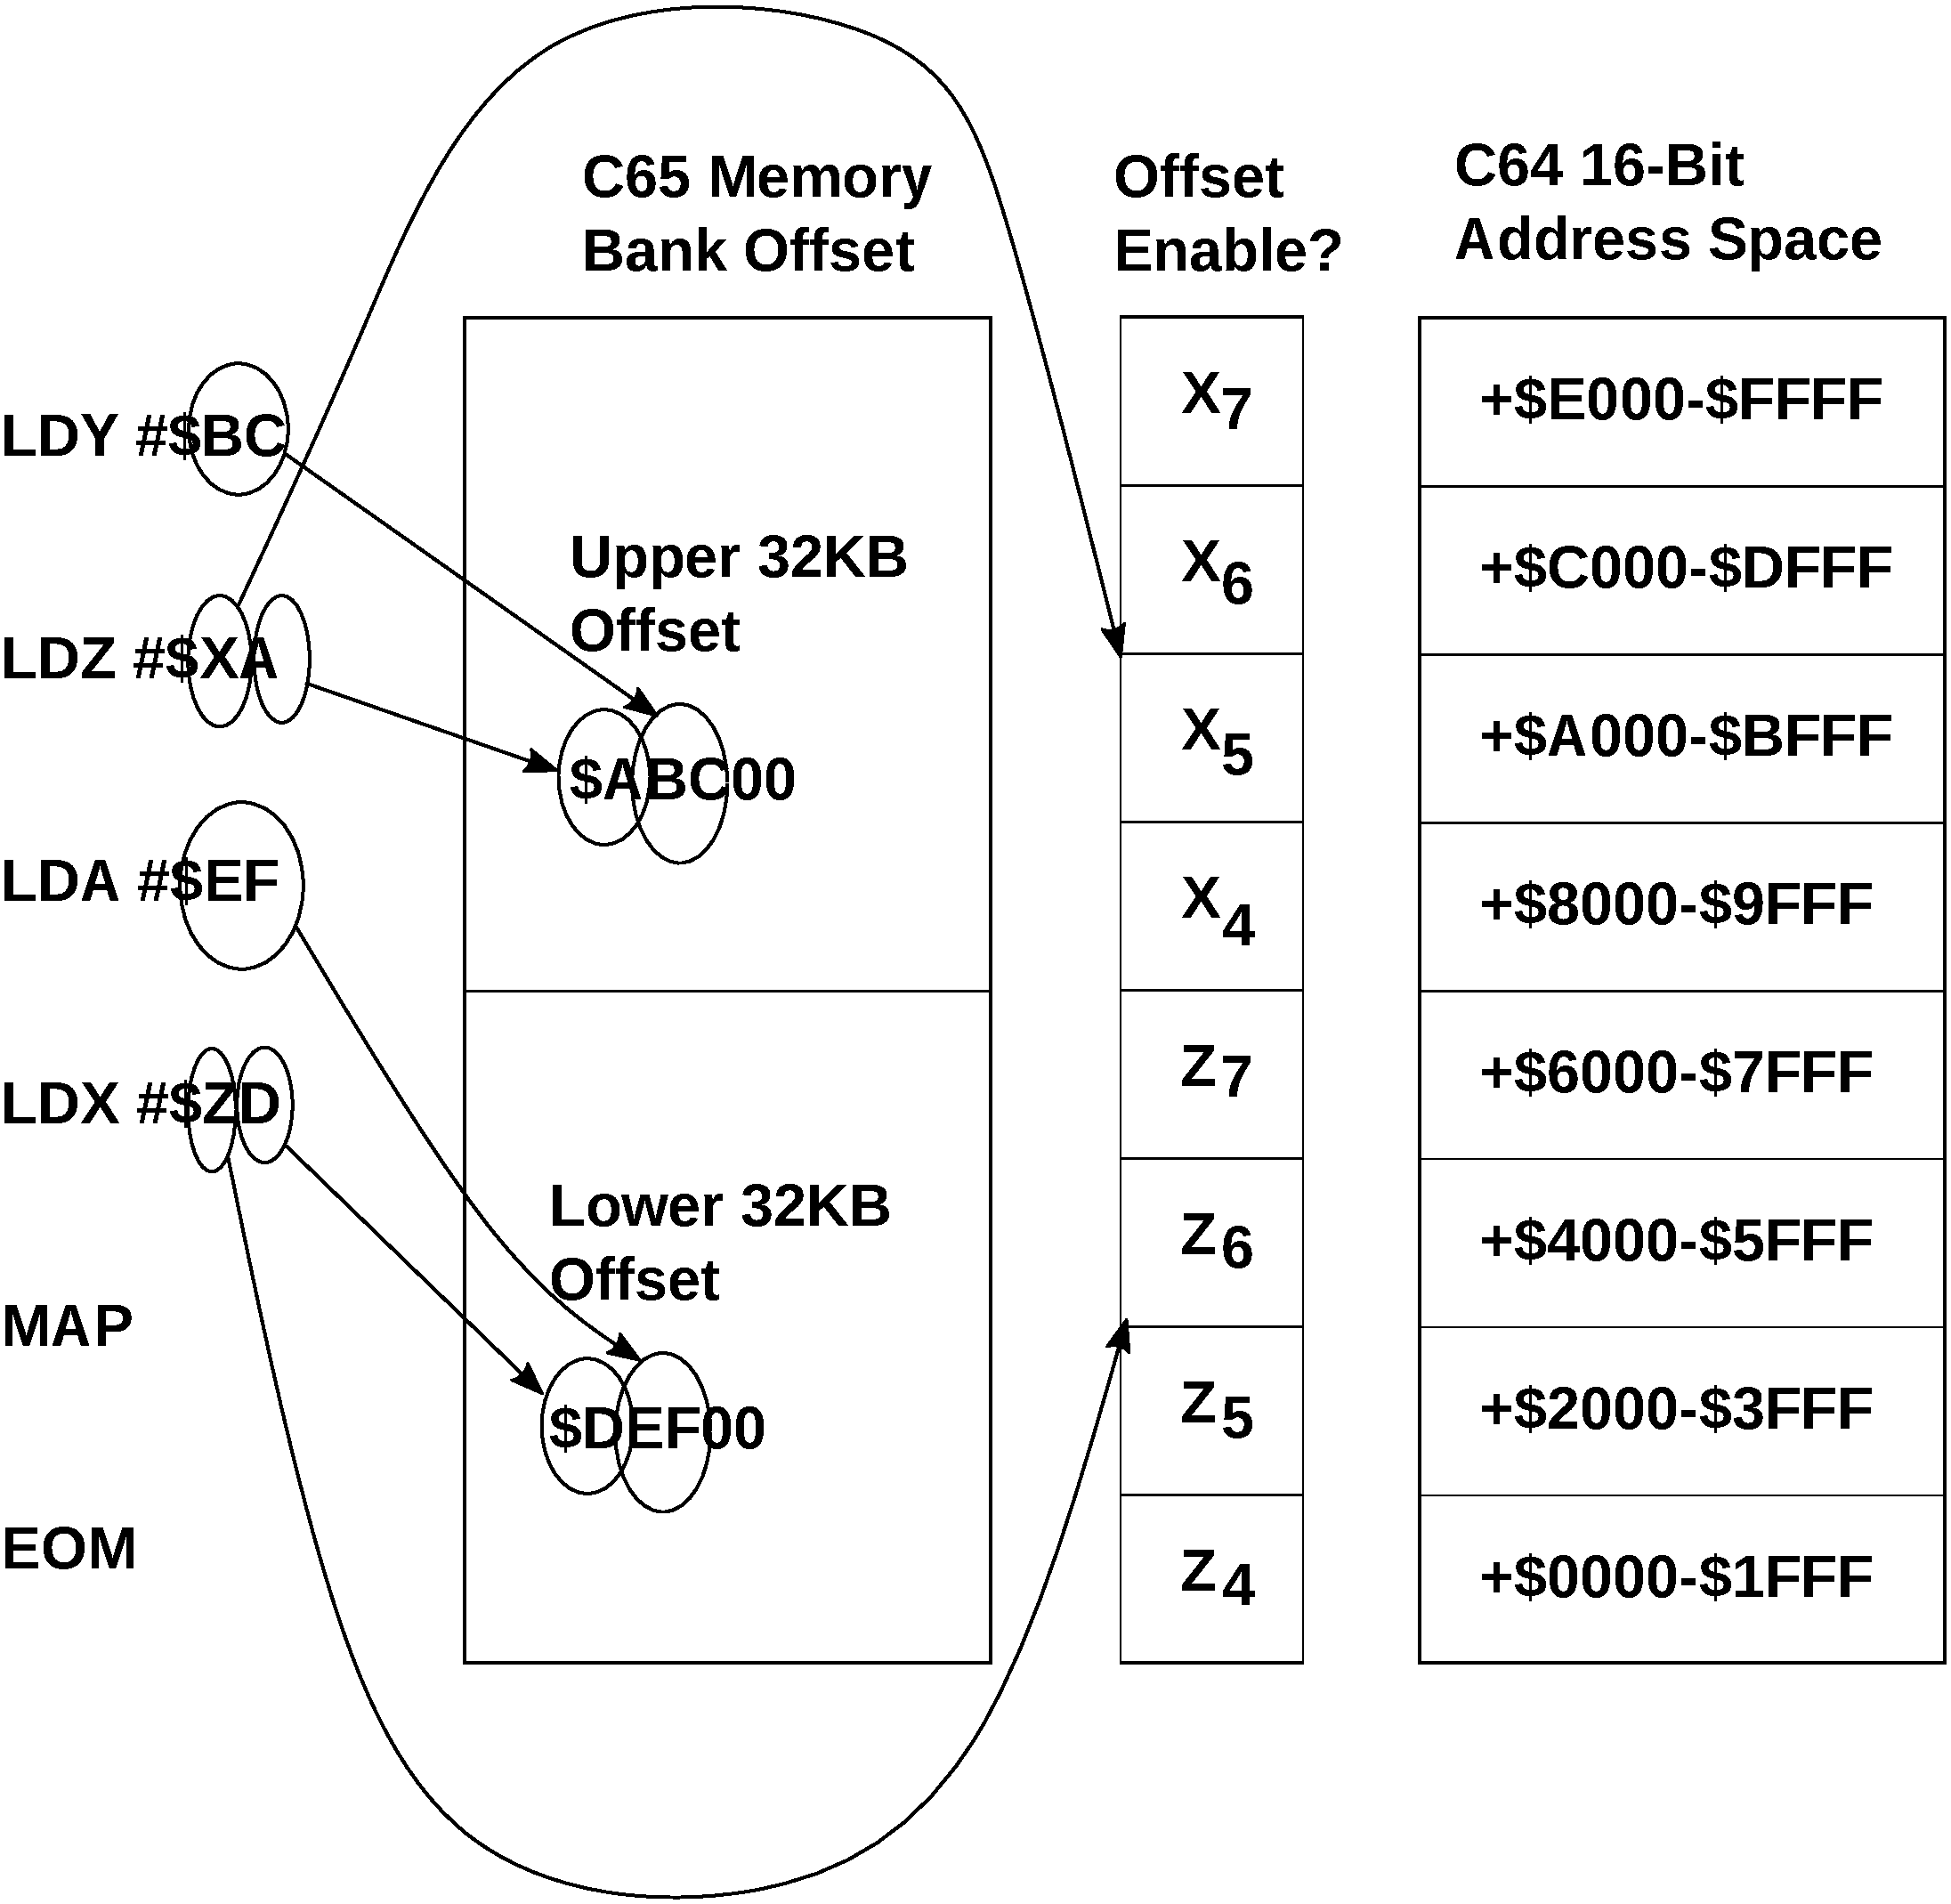
\includegraphics[width=0.75\textwidth]{images/illustrations/map-instruction-operation.pdf}\index{MAP}\index{Memory banking}
\end{center}

That is, the contents of the A register and the lower-nibble of the X register form a 12-bit value
that is multiplied by 256 to produce the offset used for any of the 8KB banks in the lower 32KB half of the 6502's 16-bit address
space.  The upper nibble of the X register is used as flags to indicate which of the four 8KB blocks in that 32KB half of the
6502 address space should have the offset added to their addresses to compute the actual address.

The Y and Z registers are used in a similar way to produce the offset for the upper 32KB half of the 6502 address space, and the
flags to indicate whether the offset is used for each of the four 8KB blocks in that half of the address space.

Note that the lower 8 bits of the offset cannot be set. That is, the offset will be a multiple of 256
bytes, unlike on some extended 6502 processors.  However, in practice this restriction is rarely
limiting.

To understand how this works in practice, the following example shows how this works with a concrete
example, showing the address ranges that would be visible in each of the 8KB slices of the 6502's
64KB address space:

\begin{center}
  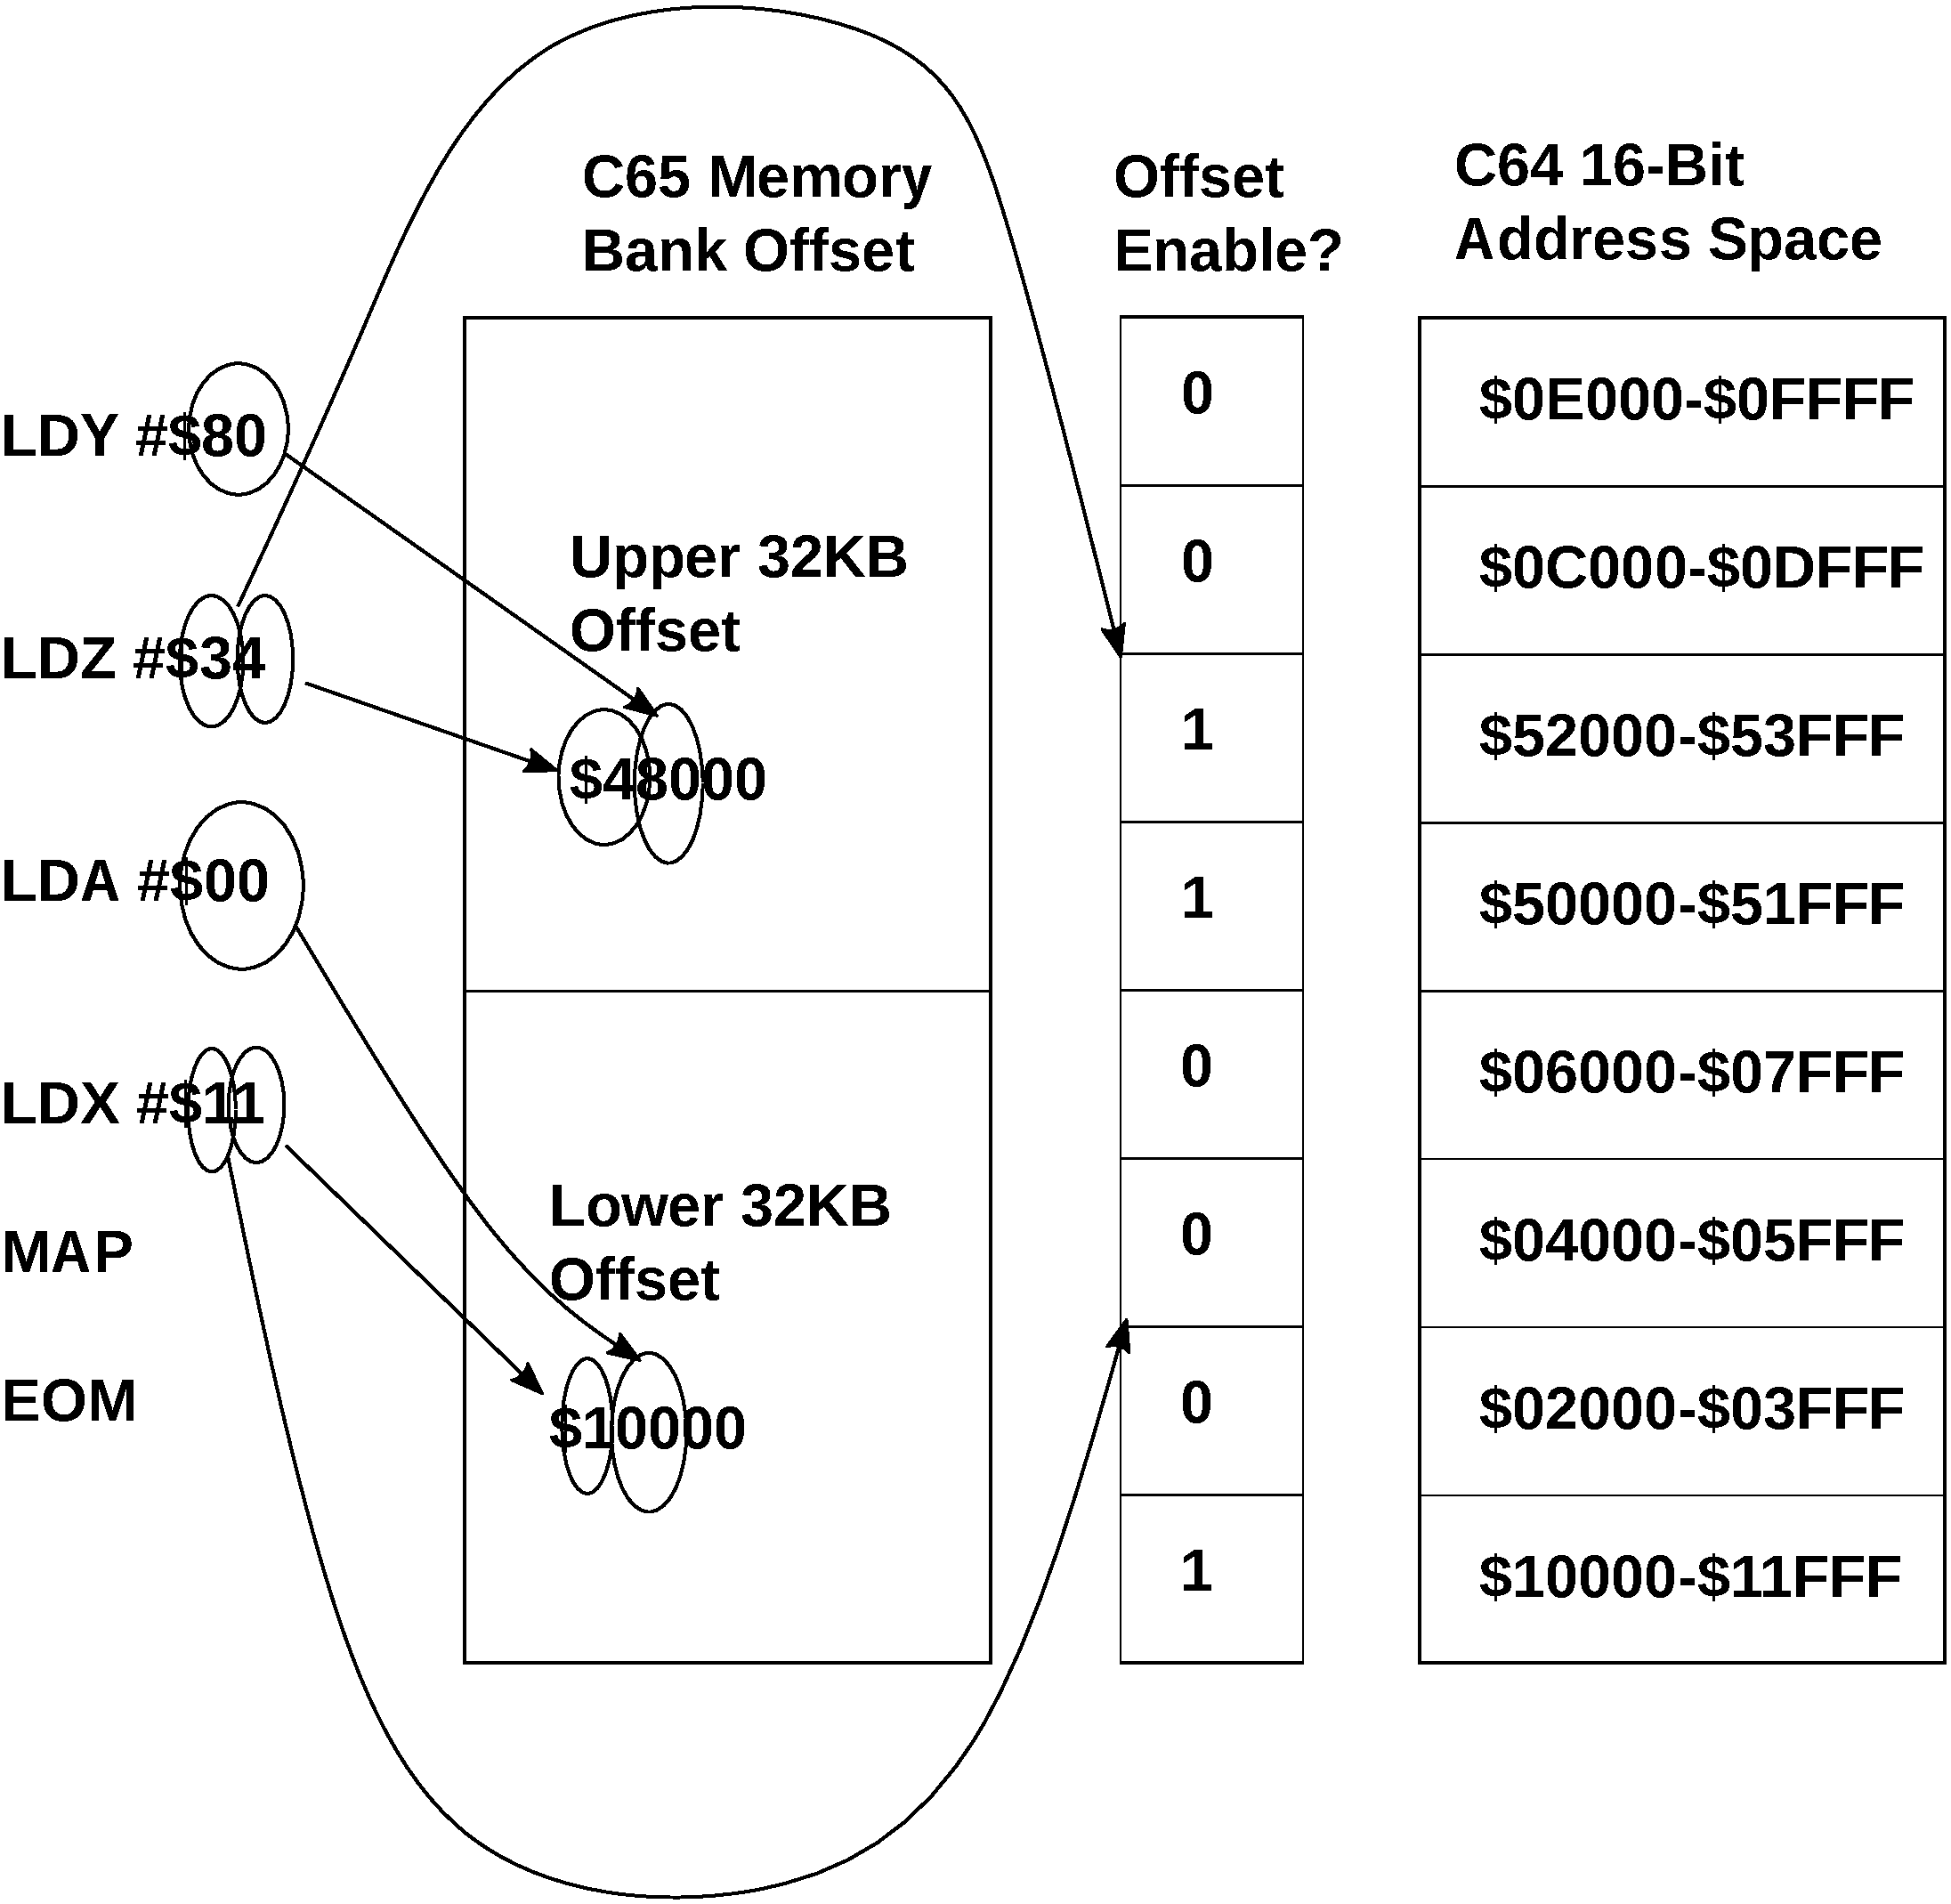
\includegraphics[width=0.75\textwidth]{images/illustrations/map-instruction-operation-example1.pdf}\index{MAP}\index{Memory banking}
\end{center}

Notice that the offsets for each of the two 32KB address ranges get added to the 6502 address.
This is why the offset of \$48000 for the upper 32KB generates an address of \$50000 at the 6502
address \$8000.

See also under ``Using the MAP instruction to access >1MB'' for further explanation.

\subsubsection{Direct Memory Access (DMA) Controller}

The C65's F018/F018A DMA controller allows for rapid filling, copying and swapping of the contents of memory
anywhere in the 1MB address space. Detailed information about the F018 DMA controller, and the MEGA65's
enhancements to this, refer to \bookvref{cha:dmagic}

\subsubsection{Flat Memory Access}

\subsection{Accessing memory beyond the 1MB point}
\label{sec:extended-memory}

The MEGA65 can support up to 256MB of memory. This is more than the 1MB address space of the CSG4510
on which it is based. There are several ways of performing this.

\subsubsection{Using the MAP instruction to access >1MB}

The full address space is available to the MAP instruction for legacy C65-style memory
mapping, although some care is required, as the MAP instruction must be called up to three times.
The reason for this is that the MAP instruction must be called to first select which mega-byte of
memory will be used for the lower and upper map regions, before it is again called in the normal
way to set the memory mapping.  Because between these two calls the memory mapping offset will be
a mix of the old and new addresses, all mapping should be first disabled via the MAP instruction.
This means that the code to re-map memory should live in the bottom 64KB of RAM or in one of the
ROM-bankable regions, so that it can remain visible during the mapping process.

Failure to handle this situation properly will result in the processor executing instructions
from somewhere unexpected half-way through the process, because the routine it is executing
to perform the mapping will suddenly no longer be mapped.

Because of the relative complexity of this process, and the other problems with the MAP instruction
as a means of memory access, we recommend that for accessing data outside of the current memory
map that you use either DMA or the flat-memory address features of the 45GS02 that are described below.
Indeed, access to the full address space via the MAP instruction is only provided for completeness.

As an other example of how the MAP instruction can be used to map an area of memory from
the expanded address space, the following program maps the Ethernet frame buffer from its natural location
at \$FFDE8000 to appear at \$6800.  To keep the example as simple as possible, we assume that the code
is running from in the bottom 64KB of RAM, and not in the region between \$6000 -- \$8000.

As the MAP instruction normally is only aware of the C65-style 20-bit addresses, the MEGA65 extension to the
instruction must be used to set the upper 8 bits of the 28-bit MEGA65 addresses, i.e., which mega-byte of address
space should be used for the address translation.  This is done by setting the X
register to \$0F when setting the mega-byte number for the lower-32KB of the C64-style 64KB address space.
This does not create any incompatibility with any sensible use of the MAP instruction on a C65, because this
value indicates that none of the four 8KB memory blocks will be re-mapped, but at the same time specifies that
the upper 4 bits of the address offset for re-mapped block is the non-zero value of \$F.  The mega-byte number
is then specified by setting the A register.

The same approach applies to the upper 32KB, but using the Z and Y
registers instead of the X and A registers.  However, in this case, we do not need to re-map the upper 32KB of
memory in this example, we will leave the Z and Y registers set to zero.  We must however set X and A to
set the mega-byte number for the lower-32KB to \$FF. Therefore A must have the value \$FF.  To set the lower 20-bits
of the address offset we use the MAP instruction a second time, this time using it in the normal C65 manner.
As we want to remap \$6800 to \$FFDE800, and have already dealt with the \$FFxxxxx offset via the mega-byte number,
we need only to apply the offset to make \$6800 point to \$DE800. \$DE800 minus \$6800 = \$D8000.  As the MAP instruction
operates with a mapping granularity of 256 bytes = \$100, we can drop the last two digits from \$D8000 to obtain the
MAP offset of \$D80. The lower 8-bits, \$80, must be loaded into the A register. The upper 4-bits, \$D, must be loaded into
the low-nibble of the X register.  As we wish to apply the mapping to only the fourth of the 8KB blocks that make up the
lower 32KB half of the C64 memory map, we must set the 4th bit of the upper nibble. That is, the upper nibble must be set
to \%1000, i.e., \$8.  Therefore the X register must be loaded with \$8D.  Thus we yield the complete example program:

\begin{tcolorbox}[colback=black,coltext=white]
\verbatimfont{\codefont}
\begin{verbatim}
; Map Ethernet registers at $6000 - $7FFF

; Ethernet controller really lives $FFDE000 - $FFDEFFF, so select $FF megabyte section for MAP LO
LDA #$ff
LDX #$0f
LDY #$00
LDZ #$00
map

; now enable mapping of $DE000-$DFFFF at $6000
; MAPs are offset based, so we need to subtract $6000 from the target address
; $DE000 - $6000 = $D8000
LDA #$80
LDX #$8d
LDY #$00
LDZ #$00
map
EOM

; Ethernet buffer now visible at $6800 - $6FFF
\end{verbatim}
\end{tcolorbox}

Note that the EOM (End Of Mapping) instruction (which is the same as NOP on a 6502, i.e., opcode \$EA) was only supplied after the last MAP instruction, to make sure that no interrupts could occur while
the memory map contained mixed values with the mega-byte number set, but the lower-bits of the mapping address had not been
updated.

No example in BASIC for the MAP instruction is possible, because the MAP is an machine code instruction of the 4510 / 45GS02 processors.

\subsubsection{Flat-Memory Access}

The 45GS02 makes it easy to read or write a byte from anywhere in memory by allowing the Zero-Page Indirect
addressing mode to use a 32-bit pointer instead of the normal 16-bit pointer.  This is accomplished by
using the Z-indexed Zero-Page Indirect Addressing Mode for the access, and having the instruction directly
preceded by a NOP instruction (opcode \$EA).  For example:

\begin{tcolorbox}[colback=black,coltext=white]
\verbatimfont{\codefont}
\begin{verbatim}
NOP
LDA ($45),Z
\end{verbatim}
\end{tcolorbox}

If you are using the ACME assembler, or another assembler that supports the 45GS02 extensions, you can instead use square-brackets
to indicate that you are performing a flat-memory operation. Such assemblers will insert the \$EA prefix automatically for you. For example:

\begin{tcolorbox}[colback=black,coltext=white]
\verbatimfont{\codefont}
\begin{verbatim}
LDA [$45],Z
\end{verbatim}
\end{tcolorbox}

Regardless which tool you are using, this example would read the four bytes of Zero-Page memory at \$45 -- \$48 to form a 32-bit memory address, and add the value of the
Z register to this to form the actual address that will be read from.  The byte order in the address is the same as
the 6502, i.e., the right-most (least significant) byte of the address will be read from the first address (\$45 in this case),
and so on, until the left-most (most significant) byte will be read from \$48.  For example, to read from memory location
\$12345678, the contents of memory beginning at \$45 should be 78 56 43 12.

This method is much more efficient and also simpler than either using the MAP instruction or the DMA controller for single memory accesses,
and is what we generally recommend.  The DMA controller can be used for moving/filler larger regions of memory.
We recommend the MAP instruction only be used for banking code, or in rare situations where extensive access to a small region of
memory is required, and the extra cycles of reading the 32-bit addresses is problematic.

\subsection{Virtual 32-bit Register}

The 45GS02 allows the use of its four general purpose registers, A, X ,Y and Z as a single virtual 32-bit register. This can greatly
simplify and speed up many common operations, and help avoid many common programming errors.
For example, adding two 16-bit or 32-bit values can now be easily accomplished with something like:

\begin{tcolorbox}[colback=black,coltext=white]
\verbatimfont{\codefont}
\begin{verbatim}
  ; Clear carry before performing addition, as normal
  CLC
  ; Prefix an instruction with two NEG instructions to select virtual 32-bit register mode
  NEG
  NEG
  LDA $1234  ; Load the contents of $1234-$1237 into A,X,Y and Z respectively
  ; And again, for the addition
  NEG
  NEG
  ADC $1238  ; Add the contents of $1238-$123B
  ; The result of the addition is now in A, X, Y and Z.
  ; And can be written out in whole or part

  ; To write it all out, again, we need the NEG + NEG prefix
  NEG
  NEG
  STA $123C ; Write the whole out to $123C-$123F

  ; Or to write out the bottom bytes, we can just write the contents of A and X as normal
  STA $1240
  STX $1241
\end{verbatim}
\end{tcolorbox}

This approach works with the LDA, STA, ADC, SBC, CMP, EOR, AND, BIT, ORA, ASL, ASR, LSR, ROL, ROR, INC and DEC instructions.
If you are using ACME or another 45GS02 aware assembler, you can instead use the new \stw{LDQ}, \stw{STQ}, \stw{ADCQ},
\stw{SBCQ}, \stw{CPQ}, \stw{EORQ}, \stw{ANDQ}, \stw{BITQ}, \stw{ORQ}, \stw{ASLQ}, \stw{ASRQ}, \stw{LSRQ}, \stw{ROLQ}, \stw{RORQ}, \stw{INQ} and \stw{DEQ}
mnemonics.\index{LDQ}\index{STQ}\index{ADCQ}\index{SBCQ}\index{CPQ}\index{EORQ}\index{ANDQ}\index{BITQ}\index{ORQ}\index{ASLQ}\index{LSRQ}\index{ROLQ}\index{RORQ}\index{INQ}\index{DEQ} The previous example would thus become:

\begin{tcolorbox}[colback=black,coltext=white]
\verbatimfont{\codefont}
\begin{verbatim}
  ; Clear carry before performing addition, as normal
  CLC
  LDQ $1234  ; Load the contents of $1234-$1237 into A,X,Y and Z respectively
  ; And again, for the addition
  ADCQ $1238  ; Add the contents of $1238-$123B
  ; The result of the addition is now in A, X, Y and Z.
  ; And can be written out in whole or part

  ; To write it all out, again, we need the NEG + NEG prefix
  STQ $123C ; Write the whole out to $123C-$123F

  ; Or to write out the bottom bytes, we can just write the contents of A and X as normal
  STA $1240
  STX $1241
\end{verbatim}
\end{tcolorbox}

The virtual 32-bit addressing mode works with any addressing mode.
However, indexed addressing modes, where X, Y or Z are added to the address should
be used with care, because these registers may in fact be holding part of a 32-bit value.

The exception is the Zero-Page
Indirect Z-Indexed addressing mode: In this case the Z register is NOT added to the target address, unlike would normally
be the case. This is to allow the virtual 32-bit register to be able to be used with flat-memory access with the combined prefix of
\stw{NEG NEG NOP},  before the instruction to allow accessing a 32-bit value anywhere in memory in a single instruction.

Note that the virtual 32-bit register cannot be used in immediate mode, e.g., to load a constant into the four general
purpose registers, or to add or subtract a constant value.  This is to
avoid problems with variable length instructions.

For LDQ and STQ, it would save at most one byte
compared to LDA \#\$nn ... LDZ \#\$nn, and would be no faster.  In fact, for many common
values, such as \#\$00000000, there are short-cuts, such as:

\begin{tcolorbox}[colback=black,coltext=white]
\verbatimfont{\codefont}
\begin{verbatim}
LDA #$00
TAX
TAY
TAZ
\end{verbatim}
\end{tcolorbox}

If you need to add or subtract a 32-bit immediate value, this may require you to re-order the arguments, or perform other
minor gymnastics.  For example, to compute the sum of the contents of memory and an immediate value, you can load the A, X, Y
and Z registers with the immediate value, and then use \stw{ADCQ} with the memory address, e.g.:

\begin{tcolorbox}[colback=black,coltext=white]
\verbatimfont{\codefont}
\begin{verbatim}
  ; Get the immediate value #$12345678 into Q
  LDA #$78
  LDX #$56
  LDY #$34
  LDZ #$12
  ; Add the contents of memory locations $1234-$1237
  NEG
  NEG
  ADC $1234
  ; Store the result back in $1234-$1237
  NEG
  NEG
  STA $1234
\end{verbatim}
\end{tcolorbox}

Again, if you are using the ACME or another 45GS02-aware assembler, this can be more compactly and
clearly written as follows. But note that in both cases the same byte-sequence of machine code is
produced, and the program will take the same number of cycles to execute.

\begin{tcolorbox}[colback=black,coltext=white]
\verbatimfont{\codefont}
\begin{verbatim}
  ; Get the immediate value #$12345678 into Q
  LDA #$78
  LDX #$56
  LDY #$34
  LDZ #$12
  ; Add the contents of memory locations $1234-$1237
  ADCQ $1234
  ; Store the result back in $1234-$1237
  STQ $1234
\end{verbatim}
\end{tcolorbox}


\section{C64 CPU Memory Mapped Registers}

\input{regtable_CPU.C64}

\section{New CPU Memory Mapped Registers}

\input{regtable_CPU.MEGA65}

\section{MEGA65 CPU Maths Acceleration Registers}

Every MEGA65 contains a combined 32-bit hardware multiplier and divider.
This device takes two 32-bit inputs, MULTINA and MULTINB, and simultaneously calculates:

\begin{itemize}
\item the 64-bit product of MULTINA and MULTINB
\item the 32-bit whole part of MULTINA / MULTINB
\item the 32-bit fractional part of MULTINA / MULTINB
\end{itemize}

It is always updating the outputs based on the inputs, so there is no need to take special action when changing the inputs.
The multiplier takes 1 cycle to calculate, and the updated result will thus be available immediately. The hardware divider,
however, can take upto 16 cycles depending on the particular inputs.  Thus programmers should insert a short delay after
changing the inputs before reading the output.  As this delay is so short, it can be implemented by simply reading the first
byte of the result four times consecutively, as the 4th read will occur after the result has settled.

Some models of the MEGA65 also include a math unit, which helps to accelerate the calculation of fixed-point formulae.
This presently disabled in all models of the MEGA65 and will be further documented if and when it becomes
available.

\input{regtable_MATH.MEGA65}

\section{MEGA65 Hypervisor Mode}
\label{sec:hypervisor-mode}

\subsection{Reset}

On power-up or reset, the MEGA65 starts up in hypervisor mode, and expects to find a program in the
16KB hypervisor memory, and begins executing instructions at address \$8100.  Normally a JMP instruction
will be located at this address, that will jump into a reset routine. That is, the 45GS02
does not use the normal 6502 reset vector. It's function is emulated by the Hyppo hypervisor program,
which fetches the address from the 6502 reset vector in the loaded client operating system when
exiting hypervisor mode.

The hypervisor memory is automatically mapped on reset to \$8000 - \$BFFF.  This special memory is not
able to mapped or in anyway accessed, except when in hypervisor mode. It can, however, always be accessed from the serial monitor/debugger
interface via its 28-bit address, \$FFF8000 -- \$FFFBFFF.  This is to protect it from accidental or malicious access from a guest operating system.

\subsection{Entering / Exiting Hypervisor Mode}

Entering the Hypervisor occurs whenever any of the following events occurs:

\begin{itemize}
\item{\bf Power-on} When the MEGA65 is first powered on.
\item{\bf Reset} If the reset line is lowered, or a watch-dog triggered reset occurs.
\item{\bf SYSCALL register accessed} The registers \$D640 - \$D67F in the MEGA65 I/O context trigger SYSCALLs when accessed.
  This is intended to be the mechanism by which a client operating system or process requests the attention of the hypervisor or operating system.
\item{\bf Page Fault} On MEGA65s that feature virtual memory, a page fault will cause a trap to hypervisor mode.
\item{\bf Certain keyboard events} Pressing \widekey{RESTORE} for >0.5 seconds, or the \specialkey{ALT} and
\specialkey{TAB} key combination traps to the hypervisor.  Typically the first is used to launch the Freeze Menu an the second to toggle the display of debug interface.
\item{\bf Accessing virtualised I/O devices} For example, if the F011 (internal 3.5'' disk drive controller) has been virtualised, then attempting to read or write sectors using this device will cause traps to the hypervisor.
  \item{\bf Executing an instruction that would lock up the CPU} A number of undocumented opcodes on the 6502 will cause the CPU to lockup.  On the MEGA65, instead of locking up, the computer will trap to the hypervisor.  This could be used to implement alternative instruction behaviours, or simply to tell the user that something bad has happened.
  \item{\bf Certain special events} Some devices can generate hypervisor-level interrupts. These are implemented as traps to the hypervisor.
\end{itemize}

The 45GS02 handles all of these in a similar manner internally:

\begin{enumerate}
\item The SYSCALL or trap address is calculated, based on the event.
\item The contents of all CPU registers are saved into the virtualisation control registers.
\item The hypervisor mode memory layout is activated, the CPU decimal flag and special purpose registers are all set to appropriate values.  The contents of the A,X,Y and Z and most other CPU flags are preserved, so that they can be accessed from the Hypervisor's SYSCALL/trap handler routine, without having to load them, thus saving a few cycles for each call.
\item The hypervisor-mode flag is asserted, and the program counter (PC) register is set to the computed address.
\end{enumerate}

All of the above happens in one CPU cycle, i.e., in 25 nano-seconds.
Returning from a SYSCALL or trap consists simply of writing to \$D67F, which
requires 125 nano-seconds, for a total overhead of 150 nano-seconds.
This gives the MEGA65 SYSCALL performance rivalling -- even beating
-- even the fastest modern computers, where the system call latency is
typically hundreds to tens of thousands of cycles \cite{soares2010flexsc}.

\subsection{Hypervisor Memory Layout}

The hypervisor memory is 16KB in size.  The first 512 bytes are
reserved for SYSCALL and system trap entry
points, with four bytes for each.  For example, the reset entry point is
at \$8100 - \$8100 + 3 = \$8100 - \$8103.
This allows 4 bytes for an instruction, typically a JMP instruction,
followed by a NOP to pad it to 4 bytes.

The full list of SYSCALLs and traps is:

\begin{longtable}{|L{1.2cm}|L{1.1cm}|C{2cm}|L{6cm}|}
\hline
{\bf{HEX}} & {\bf{DEC}} & {\bf{Name}} & {\bf{Description}} \\
\hline
\endfirsthead
\multicolumn{3}{l@{}}{\ldots continued}\\
\hline
{\bf{HEX}} & {\bf{DEC}} & {\bf{Name}} & {\bf{Description}} \\
\hline
\endhead
\multicolumn{3}{l@{}}{continued \ldots}\\
\endfoot
\hline
\endlastfoot
\small  8000 & \small 32768 & SYSCALL00 & SYSCALL 0 entry point \\
\hline
\small  8004 & \small 32772 & SYSCALL01 & SYSCALL 1 entry point \\
\hline
\small  8008 & \small 32776 & SYSCALL02 & SYSCALL 2 entry point \\
\hline
\small  800C & \small 32780 & SYSCALL03 & SYSCALL 3 entry point \\
\hline
\small  8010 & \small 32784 & SYSCALL04 & SYSCALL 4 entry point \\
\hline
\small  8014 & \small 32788 & SYSCALL05 & SYSCALL 5 entry point \\
\hline
\small  8018 & \small 32792 & SYSCALL06 & SYSCALL 6 entry point \\
\hline
\small  801C & \small 32796 & SYSCALL07 & SYSCALL 7 entry point \\
\hline
\small  8020 & \small 32800 & SYSCALL08 & SYSCALL 8 entry point \\
\hline
\small  8024 & \small 32804 & SYSCALL09 & SYSCALL 9 entry point \\
\hline
\small  8028 & \small 32808 & SYSCALL0A & SYSCALL 10 entry point \\
\hline
\small  802C & \small 32812 & SYSCALL0B & SYSCALL 11 entry point \\
\hline
\small  8030 & \small 32816 & SYSCALL0C & SYSCALL 12 entry point \\
\hline
\small  8034 & \small 32820 & SYSCALL0D & SYSCALL 13 entry point \\
\hline
\small  8038 & \small 32824 & SYSCALL0E & SYSCALL 14 entry point \\
\hline
\small  803C & \small 32828 & SYSCALL0F & SYSCALL 15 entry point \\
\hline
\small  8040 & \small 32832 & SYSCALL10 & SYSCALL 16 entry point \\
\hline
\small  8044 & \small 32836 & SECURENTR & Enter secure container trap entry point \\
\hline
\small  8048 & \small 32840 & SECUREXIT & Leave secure container trap entry point. \\
\hline
\small  804C & \small 32844 & SYSCALL13 & SYSCALL 19 entry point \\
\hline
\small  8050 & \small 32848 & SYSCALL14 & SYSCALL 20 entry point \\
\hline
\small  8054 & \small 32852 & SYSCALL15 & SYSCALL 21 entry point \\
\hline
\small  8058 & \small 32856 & SYSCALL16 & SYSCALL 22 entry point \\
\hline
\small  805C & \small 32860 & SYSCALL17 & SYSCALL 23 entry point \\
\hline
\small  8060 & \small 32864 & SYSCALL18 & SYSCALL 24 entry point \\
\hline
\small  8064 & \small 32868 & SYSCALL19 & SYSCALL 25 entry point \\
\hline
\small  8068 & \small 32872 & SYSCALL1A & SYSCALL 26 entry point \\
\hline
\small  806C & \small 32876 & SYSCALL1B & SYSCALL 27 entry point \\
\hline
\small  8070 & \small 32880 & SYSCALL1C & SYSCALL 28 entry point \\
\hline
\small  8074 & \small 32884 & SYSCALL1D & SYSCALL 29 entry point \\
\hline
\small  8078 & \small 32888 & SYSCALL1E & SYSCALL 30 entry point \\
\hline
\small  807C & \small 32892 & SYSCALL1F & SYSCALL 31 entry point \\
\hline
\small  8080 & \small 32896 & SYSCALL20 & SYSCALL 32 entry point \\
\hline
\small  8084 & \small 32900 & SYSCALL21 & SYSCALL 33 entry point \\
\hline
\small  8088 & \small 32904 & SYSCALL22 & SYSCALL 34 entry point \\
\hline
\small  808C & \small 32908 & SYSCALL23 & SYSCALL 35 entry point \\
\hline
\small  8090 & \small 32912 & SYSCALL24 & SYSCALL 36 entry point \\
\hline
\small  8094 & \small 32916 & SYSCALL25 & SYSCALL 37 entry point \\
\hline
\small  8098 & \small 32920 & SYSCALL26 & SYSCALL 38 entry point \\
\hline
\small  809C & \small 32924 & SYSCALL27 & SYSCALL 39 entry point \\
\hline
\small  80A0 & \small 32928 & SYSCALL28 & SYSCALL 40 entry point \\
\hline
\small  80A4 & \small 32932 & SYSCALL29 & SYSCALL 41 entry point \\
\hline
\small  80A8 & \small 32936 & SYSCALL2A & SYSCALL 42 entry point \\
\hline
\small  80AC & \small 32940 & SYSCALL2B & SYSCALL 43 entry point \\
\hline
\small  80B0 & \small 32944 & SYSCALL2C & SYSCALL 44 entry point \\
\hline
\small  80B4 & \small 32948 & SYSCALL2D & SYSCALL 45 entry point \\
\hline
\small  80B8 & \small 32952 & SYSCALL2E & SYSCALL 46 entry point \\
\hline
\small  80BC & \small 32956 & SYSCALL2F & SYSCALL 47 entry point \\
\hline
\small  80C0 & \small 32960 & SYSCALL30 & SYSCALL 48 entry point \\
\hline
\small  80C4 & \small 32964 & SYSCALL31 & SYSCALL 49 entry point \\
\hline
\small  80C8 & \small 32968 & SYSCALL32 & SYSCALL 50 entry point \\
\hline
\small  80CC & \small 32972 & SYSCALL33 & SYSCALL 51 entry point \\
\hline
\small  80D0 & \small 32976 & SYSCALL34 & SYSCALL 52 entry point \\
\hline
\small  80D4 & \small 32980 & SYSCALL35 & SYSCALL 53 entry point \\
\hline
\small  80D8 & \small 32984 & SYSCALL36 & SYSCALL 54 entry point \\
\hline
\small  80DC & \small 32988 & SYSCALL37 & SYSCALL 55 entry point \\
\hline
\small  80E0 & \small 32992 & SYSCALL38 & SYSCALL 56 entry point \\
\hline
\small  80E4 & \small 32996 & SYSCALL39 & SYSCALL 57 entry point \\
\hline
\small  80E8 & \small 33000 & SYSCALL3A & SYSCALL 58 entry point \\
\hline
\small  80EC & \small 33004 & SYSCALL3B & SYSCALL 59 entry point \\
\hline
\small  80F0 & \small 33008 & SYSCALL3C & SYSCALL 60 entry point \\
\hline
\small  80F4 & \small 33012 & SYSCALL3D & SYSCALL 61 entry point \\
\hline
\small  80F8 & \small 33016 & SYSCALL3E & SYSCALL 62 entry point \\
\hline
\small  80FC & \small 33020 & SYSCALL3F & SYSCALL 63 entry point \\
\hline
\small  8100 & \small 33024 & RESET & Power-on/reset entry point \\
\hline
\small  8104 & \small 33028 & PAGFAULT & Page fault entry point (not currently used) \\
\hline
\small  8108 & \small 33032 & RESTORKEY & Restore-key long press trap entry point \\
\hline
\small  810C & \small 33036 & ALTTABKEY & ALT+TAB trap entry point \\
\hline
\small  8110 & \small 33040 & VF011RD & F011 virtualised disk read trap entry point \\
\hline
\small  8114 & \small 33044 & VF011WR & F011 virtualised disk write trap entry point \\
\hline
\small  8118 & \small 33048 & BREAKPT & CPU break-point encountered \\
\hline
\small  811C -- 81FB & \small 33048 -- 33275 & RESERVED & Reserved traps point entry \\
\hline
\small  81FC & \small 33276 & CPUKIL & KIL instruction in 6502-mode trap entry point \\
\hline
\end{longtable}

The remainder of the 16KB hypervisor memory is available for use by the programmer, but
will typically use the last 512 bytes for the stack and zero-page, giving an overall memory map as follows:

\begin{longtable}{|L{1.2cm}|L{1.1cm}|L{8cm}|}
\hline
{\bf{HEX}} & {\bf{DEC}} & {\bf{Description}} \\
\hline
\endfirsthead
\multicolumn{3}{l@{}}{\ldots continued}\\
\hline
{\bf{HEX}} & {\bf{DEC}} & {\bf{Description}} \\
\hline
\endhead
\multicolumn{3}{l@{}}{continued \ldots}\\
\endfoot
\hline
\endlastfoot
\small  8000 -- 81FF & \small 32768 -- 33279 & SYSCALL and trap entry points \\
\hline
\small  8200 -- BDFF & \small 33280 -- 48639 & Available for hypervisor or operating system program \\
\hline
\small  8E00 -- BEFF & \small 48640 -- 48895 & Processor stack for hypervisor or operating system \\
\hline
\small  8F00 -- BFFF & \small 48896 -- 49151 & Processor zero-page storage for hypervisor or operating system \\
\hline
\end{longtable}

The stack is used for holding the return address of function calls.  The zero-page storage is typically used for holding
variables and other short-term storage, as is customary on the 6502.

\subsection{Hypervisor Virtualisation Control Registers}

\input{regtable_HCPU.MEGA65}

\subsection{Programming for Hypervisor Mode}

The easiest way to write a program for Hypervisor Mode on the MEGA65 is to use KickC, which is a special version of C
made for writing programs for 6502-class processors.  The following example programs are from KickC's supplied examples.
KickC produces very efficient code, and directly supports the MEGA65's
hypervisor mode quite easily through the use of a linker definition file with the following contents:

\begin{tcolorbox}[colback=black,coltext=white]
\verbatimfont{\codefont}
\begin{verbatim}
.file [name="%O.bin", type="bin", segments="XMega65Bin"]
.segmentdef XMega65Bin [segments="Syscall, Code, Data, Stack, Zeropage"]
.segmentdef Syscall [start=$8000, max=$81ff]
.segmentdef Code [start=$8200, min=$8200, max=$bdff]
.segmentdef Data [startAfter="Code", min=$8200, max=$bdff]
.segmentdef Stack [min=$be00, max=$beff, fill]
.segmentdef Zeropage [min=$bf00, max=$bfff, fill]
\end{verbatim}
\end{tcolorbox}

This file instructs KickC's assembler to create a 16KB file with the 512 byte SYSCALL/trap entry point region at the start,
followed by code and data areas, and then the stack and zero-page areas. It enforces the size and location of these fields, and
will give an error during compilation if anything is too big to fit.

With this file in place, you can then create a KickC source file that provides data structures for the SYSCALL/trap table, e.g.:

\begin{tcolorbox}[colback=black,coltext=white]
\verbatimfont{\codefont}
\begin{verbatim}
// XMega65 KERNAL Development Template
// Each function of the KERNAL is a no-args function
// The functions are placed in the SYSCALLS table surrounded by JMP and NOP

import "string"

// Use a linker definition file (put the previous listing into that file)
#pragma link("mega65hyper.ld")

// Some definitions of addresses and special values that this program uses
const char* RASTER = 0xd012;
const char* VIC_MEMORY = 0xd018;
const char* SCREEN = 0x0400;
const char* BGCOL = 0xd021;
const char* COLS = 0xd800;
const char BLACK = 0;
const char WHITE = 1;

// Some text to display
char[] MESSAGE = "hello world!";

void main() {
    // Initialise screen memory, and select correct font
    *VIC_MEMORY = 0x14;
    // Fill the screen with spaces
    memset(SCREEN, ' ', 40*25);
    // Set the colour of every character on the screen to white
    memset(COLS, WHITE, 40*25);
    // Print the "hello world!" message
    char* sc = SCREEN+40;  // Display it one line down on the screen
    char* msg = MESSAGE; // The massage to display
    // A simple copy routine to copy the string
    while(*msg) {
        *sc++ = *msg++;
    }
    // Loop forever showing two white lines as raster bars
    while(true) {
        if(*RASTER==54 || *RASTER==66) {
            *BGCOL = WHITE;
        } else {
            *BGCOL = BLACK;
        }
    }
}

// Here are a couple sample SYSCALL handlers that just display a character on the screen
void syscall1() {
    *(SCREEN+79) = '>';
}

void syscall2() {
    *(SCREEN+78) = '<';
}

// Now we select the SYSCALL segment to hold the SYSCALL/trap entry point table.
#pragma data_seg(Syscall)

// The structure of each entry point is JMP <handler address> + NOP.
// We have a char (xjmp) to hold the opcode for the JMP instruction,
// and then put the address of the SYSCALL/trap handler in the next
// two points as a pointer, and end with the NOP instruction opcode.
struct SysCall {
    char xjmp;         // Holds $4C, the JMP $nnnn opcode
    void()* syscall;   // Holds handler address, will be the target of the JMP
    char xnop;         // Holds $EA, the NOP opcode
};

// To save writing 0x4C and 0xEA all the time, we define them as constants
const char JMP = 0x4c;
const char NOP = 0xea;

// Now we can have a nice table of up to 64 SYSCALL handlers expressed
// in a fairly readable and easy format.
// Each line is an instance of the struct SysCall from above, with the JMP
// opcode value, the address of the handler routine and the NOP opcode value.
export struct SysCall[] SYSCALLS = {
    { JMP, &syscall1, NOP },
    { JMP, &syscall2, NOP }
    };

// In this example we had only two SYSCALLs defined, so rather than having
// another 62 lines, we can just ask KickC to make the TRAP table begin
// at the next multiple of $100, i.e., at $8100.
export align(0x100) struct SysCall[] SYSCALL\_RESET = {
    { JMP, &main, NOP }
};
\end{verbatim}
\end{tcolorbox}

If you save the first listing into a file called mega65hyper.ld, and the second
into a file called mega65hyper.kc, you can then compile them using KickC with
a command like:

\begin{tcolorbox}[colback=black,coltext=white]
\verbatimfont{\codefont}
\begin{verbatim}
  kickc -a mega65hyper
\end{verbatim}
\end{tcolorbox}

It will then produce a file called mega65hyper.bin, which you can then try out
on your MEGA65, or run in the XMega65 emulator with a command like:

\begin{tcolorbox}[colback=black,coltext=white]
\verbatimfont{\codefont}
\begin{verbatim}
  xmega65 -kickup mega65hyper.bin
\end{verbatim}
\end{tcolorbox}
